\documentclass{article} %tipo del documento
\usepackage{fontspec} %font times new roman
\usepackage{listings} %pacchetto per il codice

\setmainfont{Times New Roman}
\usepackage{setspace} %interlinea singola
\singlespacing 
\usepackage[a4paper,top=2cm,bottom=3cm,left=2cm,right=2cm, heightrounded, bindingoffset=0mm]{geometry} %margini 2 cm


\usepackage{listings}
\usepackage{color}

\definecolor{dkgreen}{rgb}{0,0.6,0}
\definecolor{gray}{rgb}{0.5,0.5,0.5}
\definecolor{mauve}{rgb}{0.58,0,0.82}

\lstset{frame=tb,
  language=Java,
  aboveskip=3mm,
  belowskip=3mm,
  showstringspaces=false,
  columns=flexible,
  basicstyle={\small\ttfamily},
  numbers=none,
  numberstyle=\tiny\color{gray},
  keywordstyle=\color{blue},
  commentstyle=\color{dkgreen},
  stringstyle=\color{mauve},
  breaklines=true,
  breakatwhitespace=true,
  tabsize=3
}


\title{Relazione Progetto WORTH Reti}
\author{Lorenzo Angeli - Corso A - 539036}
\date{2020/2021}
\usepackage{graphicx}
\graphicspath{ {./Foto1/} }

\begin{document}

\maketitle

\section{Introduzione}
L’architettura di Worth è costituita da due componenti principali: il Client e il Server.
L'immagine sottostante rappresenta in modo molto semplice il funzionamento. Il Client tramite linea di comando riceve dei messaggi. Questi, se sono corretti, vengono filtrati ed inviati al Server che gli elaborerà e risponderà al Client. Lo scambio dei messaggi tra Client e Server avviene utilizzando il protocollo TCP, utilizzato per lo scambio dei comandi principali. Per i comandi di {\itshape readchat} e {\itshape sendchatmsg} si utilizza invece un'architettura diversa portando al minimo l'interazione tra il Client e il Server.
\begin{figure}[h]
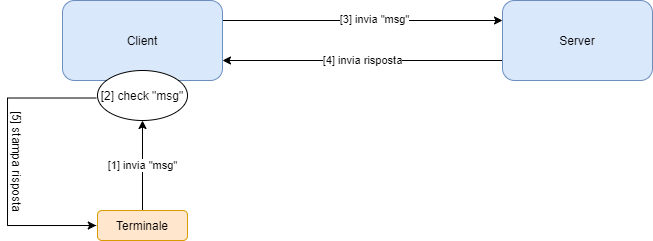
\includegraphics[width=16cm]{Foto1}
\caption{Rappresentazione semplificata dell'architettura di WORTH.}
\label{fig:sidecap}
\end{figure}
\subsection{Schema dei Thread attivati}
\begin{itemize}
    \item Il {\itshape Server} oltre al thread main attiva un thread (sempre attivo) all'avvio che rimane in attesa per accettare nuove connessioni TCP dal client. Per ogni connessione accettata avvia un thread per lo scambio di messaggi con il client. Il Server avvia poi anche un thread (sempre attivo) che crea un gruppo multicast e vi rimane collegato. Infine attiva il thread demone di RMI che rimane in attesa di invocazione di metodi remoti.
    \item Il {\itshape Client} oltre al thread main all'avvio crea un thread (sempre attivo) che intercetta i pacchetti sul gruppo multicast.
\end{itemize}
\section{Server}
Il Server utilizza un pool di thread di tipo newFixedThreadPool (max\_thread\_active) con max\_thread\_active impostato a 20 di default ma il cui valore può essere modificato accedendo al codice della classe ServerTCP. Quest'ultima classe si occupa dell'instaurazione delle nuove connessioni TCP con i Client. Il Server viene avviato tramite {\itshape MainServer.java}. Per funzionare ha a disposizione alcune classi elencate di seguito:
\begin{enumerate} 
\item Classi usate per implementare le strutture dati:
	\begin{itemize} 
	\item Progetto
	\item Utente
	\item Card
	\item Messaggi
	\item OnlineUsers
	\end{itemize} 
\item Classi/Interfacce per implementare l'RMI Register (vedi sezione RMI Register):
	\begin{itemize} 
	\item IRegister -> Interfaccia
	\item RMIServerRegister -> Classe
	\end{itemize}
\item Classi/Interfacce per implementare l'RMI CallBack (vedi sezione RMI CallBack):
	\begin{itemize} 
	\item INotify -> Interfaccia
	\item RMIServerNotify -> Classe
	\end{itemize} 
\item Classi usate per gestire i messaggi TCP: 
	\begin{itemize} 
	\item TaskConnectionTCP
	\item ServerTCP
	\end{itemize} 
\item Classi usate per gestire la chat UDP Multicast (vedi sezione Chat UDP Multicast)):
	\begin{itemize} 
	\item ServerMulticast
	\end{itemize} 
\end{enumerate}
\subsection{Breve descrizione delle classi principali viste sopra}
\subsubsection{Progetto}
La classe Progetto utilizza le seguenti variabili e strutture dati:
\begin{lstlisting}
private String nameproject;
private ConcurrentLinkedQueue <String> listamembri; //membri che partecipano al progetto
private ConcurrentLinkedQueue <Card> listatodo; //lista todo
private ConcurrentLinkedQueue <Card> listainprogress; //lista inprogress
private ConcurrentLinkedQueue <Card> listatoberevised; //lista toberevised
private ConcurrentLinkedQueue <Card> listadone; //lista done
\end{lstlisting}
Questa classe è utile per memorizzare il contenuto di un progetto. Per memorizzare le carte ho utilizzato quattro liste di Card, ogni lista contiene le carte di un determinato stato (todo, inprogress, toberevised, done).
\subsubsection{Card}
La classe Card utilizza le seguenti variabili e strutture dati:
\begin{lstlisting}
private String name; //nome della carta
private String description; //descrizione della carta
private int state; //stato della carta (stato compreso tra 0 e 3)
private ConcurrentLinkedQueue<Integer> historylist = new ConcurrentLinkedQueue<Integer>();
\end{lstlisting}
dove {\itshape state} contiene lo stato attuale della carta (compreso tra 0 e 3). Se state=0 allora la carta si trova nello stato "todo"; se state=1 si trova nello stato "inprogress"; se state=2 si trova nello stato "toberevised"; se state=3 si trova nello stato "done". La {\itshape historylist} contiene una lista di interi, ogni intero è compreso tra 0 e 3 e rappresenta un particolare stato della carta. E' di particolare importanza che l'ordine di questa lista venga mantenuto.
\subsubsection{Utente}
La classe Utente utilizza le seguenti variabili:
\begin{lstlisting}
private String username; //nome utente
private String password; //password utente
\end{lstlisting}
\subsubsection{Messaggi}
La classe Messaggi utilizza la seguente variabile e struttura dati: 
\begin{lstlisting}
private String nameproject;
private ConcurrentLinkedQueue<String> msglist;
\end{lstlisting}
Viene utilizzata in WORTH per contenere una lista di messaggi relativi ad un progetto. Si utilizza lato Client per memorizzare i messaggi intercettati da ThreadSniffing (classe che vedremo più avanti).
\subsubsection{OnlineUsers}
La classe OnlineUsers contiene la seguente struttura dati: 
\begin{lstlisting}
private ConcurrentHashMap<String,Integer> onlineusers;
\end{lstlisting}
che servono a memorizzare i nickname degli utenti online. Questa classe viene usata lato Server dalla classe RMIServerNotify per passare gli utenti online al Client, usando il meccanismo di serializzazione dell'oggetto (marshalling). 
\subsection{Organizzazione di File e Cartelle su disco}
All'interno della directory principale del programma vengono create due cartelle: Progetti e Utenti. 
\begin{itemize}
    \item La cartella "Progetti" contiene al proprio interno altre eventuali cartelle, ognuna di queste cartelle si riferisce ad un progetto creato e prende il nome di tale progetto. All'interno di una cartella riferita ad uno specifico progetto sono presenti due file: una cartella "Card" e un file di testo "listamembri.txt". Il file di testo contiene la lista dei membri che fanno parte del progetto. La cartella "Card" contiene dei file in formato json, ognuno inerente ad una carta creata.
    \item La cartella "Utenti" contiene al proprio interno tante cartelle quanti sono gli utenti registrati al servizio WORTH. Ogni cartella (che esiste solo se l'utente è registrato) prende il nome del nickname dell'utente che ha creato l'account (l'utente rappresentato dal nickname "pippo" avrà una cartella chiamata "pippo"). All'interno di questa cartella è presente il file "login.json" che contiene le credenziali dell'utente inserite al momento della registrazione del suo account. 
\end{itemize}
\section{Client}
Il Client viene avviato tramite {\itshape MainClient.java}. Vediamo di seguito lo pseudocodice di questa classe per capire meglio l'architettura:
\begin{lstlisting}
while (true) {
   String read_console = in.nextLine(); //leggo da tastiera il comando digitato dall'utente
	String ar [] = read_console.split(" ");
	String comando = ar[0];
	
	if (comando.contentEquals("register")) {
	    ...
	}
	else if (comando.contentEquals("login")) {
	    ...
	}
	...
	...
}
\end{lstlisting}
Per funzionare, il Client ha a disposizione alcune classi elencate di seguito:
\begin{enumerate} 
\item Classi usate per implementare le strutture dati:
	\begin{itemize} 
	\item Progetto
	\item Utente
	\item Card
	\item Messaggi
	\end{itemize} 
\item Classi usate per gestire i messaggi TCP:
	\begin{itemize}
	\item ClientTCP
	\end{itemize}
\item Classi usate per gestire la chat UDP Multicast (vedi sezione Chat UDP Multicast):
	\begin{itemize}
	\item ClientUDP
	\item ThreadSniffing
	\end{itemize}
\item Classi/Interfacce usate per implementare l'RMI CallBack (vedi sezione RMI CallBack)
	\begin{itemize}
	\item NotifyEventInterface -> Interfaccia
	\item NotifyEventImpl -> Classe
	\end{itemize}
\end{enumerate}
\section{Scambio messaggi TCP client-server}
Lo scambio di messaggi tra il Client e il Server è molto importante.
Quasi ogni comando digitato dal terminale Client passa per quello Server utilizzando una connessione TCP. Un Client non appena esegue il comando di {\itshape login} apre una connessione TCP stabile che verrà chiusa solamente dopo aver chiuso il client. Il Server analizza il comando ricevuto facendo lo split del messaggio, lo fa elaborare dal giusto metodo e restituisce un messaggio da inoltrare poi al Client (utilizzando la connessione TCP). Per semplicità occupiamoci prima dell'architettura lato Server e dopo di quella Client.
\begin{itemize}
    \item Lato Server ho utilizzato due classi: ServerTCP e TaskConnectionTCP. {\itshape ServerTCP} attiva un thread (sempre attivo) che si occupa di accettare nuove richieste di connessione TCP dai client. Dopo aver accettato una nuova connessione avvia un Task di tipo TaskConnectionTCP che gestirà la connessione. Il codice della run() di questo Task rimane sempre in ascolto di nuovi messaggi inviati dal client (thread sempre attivo). Non appena ne riceve uno, effettua un parsing e lo smista alla porzione di codice apposita per quel particolare comando.
    \item Lato Client si fa affidamento alla classe {\itshape ClientTCP}. E' questa classe che effettua la vera e propria comunicazione con il Server. Il MainClient dopo aver acquisito la lettura del comando da terminale lo fa "matchare" all'if appropriato. Nel caso sia un comando che prevede una comunicazione con il client chiama il metodo appropriato dalla classe ClientTCP. Infatti questa classe ha un metodo per ogni tipo di comando implementato ad eccezione dei comandi per la chat di progetto (quelli vengono gestiti dalla classe ClientUDP).
\end{itemize}
\section{Chat UDP Multicast}
La Chat è stata implementata utilizzando UDP Multicast. Il Server appena avviato crea un oggetto di tipo ServerMulticast. La classe ServerMulticast implementa Runnable e ci consente di poter utilizzare l'oggetto creato come Task. Il metodo run() di tale classe non fa altro che creare un gruppo Multicast all'indirizzo 226.226.226.226 e registrarsi a tale gruppo, questo per evitare che il gruppo venga eliminato in mancanza di utenti. Il Client che scrive nella chat non fa altro che inviare un pacchetto al gruppo Multicast di indirizzo 226.226.226.226. Il Client utilizza una classe ThreadSniffing che implementa Runnable e questo ci consente di creare un Task e di poterlo avviare da un thread. Questo Task si registra al Multicast (si aggiunge al gruppo) e rimane in attesa dei pacchetti che arrivano. Appena ne arriva uno lo inserisce nella struttura dati ConcurrentHashMap<String, Messaggi> msglist che ha come chiave il nome del progetto e come argomento i messaggi della chat associati a tale chiave. Ovviamente la struttura dell'utente che ha scritto il messaggio nella chat di progetto non dovrà aggiungere alcun nuovo messaggio. Il messaggio verrà aggiunto nella struttura degli altri utenti che hanno avviato il {\itshape MainClient.java}. Nella struttura di ogni utente vengono salvati tutti i messaggi qualsiasi sia il progetto di cui fa parte tale utente. Si occuperà poi il metodo associato alla richiesta di lettura dei messaggi di dare o meno la possibilità di farglieli leggere. Se l'utente è loggato e fa parte del progetto di cui vuole leggere la chat non avrà problemi a poterlo fare. Non vale la stessa cosa per gli utenti non loggati o che non fanno parte del progetto.  
\section{RMI Register}
La fase di registrazione di un utente al servizio WORTH è stata eseguita rispettando i requisiti richiesti dal testo del progetto utilizzando RMI (Remote Method Invocation). 
\begin{itemize} 
    \item Lato Client è stato creato un "rappresentante del server" (stub o proxy) chiamato {\itshape serverObject}. Con questo oggetto dal client si possono chiamare i metodi dell'oggetto come se fossero locali anche se si trovano sul Server. Il metodo in questione si chiama {\itshape register} la cui interfaccia è "int register (String nickUtente, String password) throws RemoteException" ed è presente nell'interfaccia {\itshape IRegister}. L'oggetto viene chiamato nella fase di login dal client e restituisce un valore intero uguale a 0 se la registrazione è andata a buon fine. 
    \item Lato Server per gestire l'RMI Register viene utilizzata la classe {\itshape RMIServerRegister}. Questa classe implementa Runnable e contiene il metodo per registrare un utente al servizio WORTH, inoltre la classe si occupa di creare un file nella cartella "Utenti" e il suo file "login.json". Si scrive sul file "login.json" con una procedura di serializzazione che fa uso di un ObjectMapper. Questo sfrutta l'oggetto di tipo Utente creato poco prima, inizializzato con le credenziali dell'utente appena registrato. Oltre a questo processo si inserisce anche questo oggetto di tipo Utente nella lista concorrente ConcurrentLinkedQueue<Utente> listuseregister per mantenere aggiornata la lista degli utenti registrati al servizio WORTH. 
\end{itemize} 
\section{RMI CallBack}
La CallBack è utile quando un Client è interessato allo stato di un oggetto remoto e vuole ricevere una notifica asincrona quando lo stato viene modificato. Utilizzare lo strumento di RMI CallBack ci semplifica l'aggiornamento degli stati degli utenti (online/offline) mantenendo aggiornata la lista "listuseronline" presente nel {\itshape MainClient}. Vediamo le scelte di implementazione in questa sezione parlando prima delle scelte lato Client e dopo lato Server.
\begin{itemize}
    \item Lato Client viene utilizzata un'interfaccia e una classe. L'interfaccia {\itshape NotifyEventInterface} contiene la dichiarazione del solo metodo "void notifyEvent(OnlineUsers onlineusers)". Questo è il metodo usato dal server per la notifica al client di una nuova modifica dello stato di un utente. La classe {\itshape NotifyEventImpl} è la classe che estende RemoteObject e implementa NotifyEventInterface, ha quindi l'implementazione vera e propria del metodo NotifyEvent. Tale metodo ha un argomento, questo viene passato dal server al client usando il meccanismo di serializzazione dell'oggetto (marshalling). L'oggetto passato contiene l'intera lista dello stato degli utenti aggiornata che servirà al client per aggiornare la propria. La fase di iscrizione alla ricezione degli eventi viene fatta dopo il login dell'utente e quella di disiscrizione dopo il logout utilizzando rispettivamente i metodi registerForCallBack e unregisterForCallBack (metodi implementati lato server).
    \item Lato Server viene utilizzata un'interfaccia e una classe. L'interfaccia {\itshape INotify} contiene la dichiarazione dei metodi "void registerForCallback (NotifyEventInterface ClientInterface, String nickname)" e "public void unregisterForCallback (NotifyEventInterface ClientInterface, String nickname)" utili al client per iscriversi e disiscriversi al servizio di notifica. La classe {\itshape RMIServerNotify} contiene invece l'implementazione dei due metodi appena citati ma anche altri. Ha il metodo "public void update (OnlineUsers onlineusers)" che notifica la variazione di stato da parte di un utente registrato (quando viene chiamato manda una callback a tutti i client registrati al sistema di notifica). Per sapere quali sono gli utenti registrati al sistema di notifica viene usata una lista "private List <NotifyEventInterface> clients;" che aggiunge un cliente ogni qualvolta viene fatta una nuova registrazione alla callback e lo rimuove di conseguenza ad una disiscrizione. L'ultimo metodo è "public void fix\_unregisterForCallback (String nickname)", andiamo ad analizzare la sua funzione. Il programma WORTH non implementa un sistema di chiusura del terminale client tramite linea di comando. Per questo motivo è necessario gestire la chiusura del terminale come se fosse una chiusura improvvisa. Essendo il client ad occuparsi della fase di disiscrizione al servizio di callback in caso di chiusura improvvisa di questo, è il server che dovrà gestirla. Deve quindi rimuovere dalla lista "clients" l'oggetto associato all'utente disconnesso. Utilizza la struttura "private ConcurrentHashMap<String, NotifyEventInterface> map;" che lega il nome del client registrato alla callback con lo stub associato ed è utile per disiscrivere un utente dal sistema di notifiche in caso di disconnessione improvvisa. Si va a cercare lo stub nella hashmap "map" e si rimuove il cliente dalla lista "clients".
\end{itemize}
\section{Json - serializzazione e deserializzazione}
In vari punti del codice è stata fatta la serializzazione e deserializzazione di alcuni oggetti Json utilizzando la libreria "Jackson Json - versione 2.11.1" vista a lezione. In particolare la classe Card, OnlineUsers e Utente implementano tutte quante l'interfaccia Serializable. Questo semplifica il salvataggio su disco delle credenziali degli utenti registrati (classe Utente), delle carte associate ad un progetto (classe Card) e il passaggio della struttura contenente gli utenti online dal server al client sfruttando RMI CallBack (classe OnlineUsers). Rende infine più semplice il ripristino della consistenza delle strutture dati dopo un riavvio del Server.

\section{Lista Comandi}
Di seguito vediamo uno schema con la lista dei comandi implementati che possono essere usati lato Client. \\

\hspace{-1.7 cm}
\begin{tabular}{|l|c|c|}
\hline
\multicolumn{3}{|c|}{}\\
\multicolumn{3}{|c|}{\textbf{\Large Comandi}}\\
\multicolumn{3}{|c|}{}\\
\hline
\multicolumn{1}{|c|}{\textbf{Comando}} & \textbf{Sintassi} &
\multicolumn{1}{c|}{\textbf{Esempio}}\\
\hline
register & register <nickname> <password>  & register Luca qwerty \\
login & login <nickname> <password> & login Luca qwerty \\
listusers & listusers & listusers \\
listonlineusers & listonlineusers & listonlineusers \\
create\_project & create\_project <projectname> & create\_project Progetto1 \\
add\_member & add\_member <projectname> <member> & add\_member Progetto1 Mario \\
listprojects & listprojects & listprojects \\
showmembers & showmembers <projectname> & showmembers Progetto1 \\
add\_card & add\_card <projectname> <cardname> <carddescription> & add\_card Progetto1 Card descrizione \\
showcards & showcards <projectname> & showcards Progetto1 \\
showcard & showcard <projectname> <cardname> & showcard Progetto1 Card \\
movecard & movecard <projectname> <cardname> <listap> <listad> & movecard Progetto1 Card todo inprogress \\
getcardhistory & getcardhistory <projectname> <cardname> & getcardhistory Progetto1 Card \\
readchat & readchat <projectname> & readchat Progetto1 \\
sendchatmsg & sendchatmsg <projectname> & sendchatmsg Progetto1 \\
cancel\_project & cancel\_project <projectname> & cancel\_project Progetto1 \\
logout & logout & logout \\
\hline
\end{tabular}
\subsection{Comandi nel dettaglio}
\begin{itemize}
    \item register <nickname> <password>: la registrazione di un nuovo utente avviene tramite RMI, invocando il metodo remoto register (nickname, password) presente sul Server, che crea un file <nickname>.json in questo modo: {\itshape Utenti/<nickname>.json}. Il seguente file viene generato tramite una serializzazione (usando la Libreria Jackson) da Java to Json. L'oggetto Java da serializzare è di tipo Utente. Prima di effettuare l'operazione vera e propria si effettua un controllo per verificare che l'utente non sia già stato registrato in precedenza.
    \item login <nickname> <password>: la fase di login può avvenire solo dopo aver registrato il proprio account mediante comando register. Il client si registra anche ad un sistema di notifiche CallBack che lo aggiorna sullo stato degli utenti (online/offline).
    \item listusers: questo comando viene eseguito solo e soltanto dopo aver effettuato il login dell'utente. Stampa gli utenti registrati associando ad ognuno di essi uno stato (online/offline). Per determinare lo stato si fa affidamento alla struttura dati "listuseregister" che viene aggiornata ogni qual volta vada utilizzata.
    \item listonlineusers: comando molto simile a quello appena visto sopra ma con la differenza che in questo caso vengono stampati solo i nickname degli utenti online.
    \item create\_project <projectname>: comando utilizzato per creare un nuovo progetto; è necessario che l'utente abbia fatto il login. Ogni progetto è univoco.
    \item add\_member <projectname> <member>:  comando per aggiungere un nuovo utente ad un progetto specifico. L'utente da aggiungere deve essere stato creato precendemente. 
    \item listprojects: restituisce la lista dei progetti creati.
    \item showmembers <projectname>: restituisce la lista dei membri che fanno parte di un particolare progetto. Tramite comunicazione TCP con il Server il Client riceve la lista aggiornata dei membri del progetto <projectname>. 
    \item add\_card <projectname> <cardname> <carddescription>:  in questo comando il Client non fa altro che inviare al Server una stringa "add\_card <projectname> <cardname> <carddescription> <nickname>" tramite connessione TCP e lascerà gestire tutto a lui. Ovviamente riceverà un messaggio di successo o di un particolare errore riscontrato durante la procedura di creazione della carta. La stringa inviata al Server contiene anche il <nickname> dell'utente che vuole aggiungere la carta. Questo perchè il Server deve controllare che l'utente sia un membro del progetto.
    \item showcards <projectname>: in questo comando il Client non fa altro che inviare al Server una stringa "showcards <projectname> <nickname>" tramite connessione TCP. La stringa inviata al Server contiene anche il <nickname> dell'utente che vuole visionare le carte. Questo perchè il Server deve controllare che l'utente sia un membro del progetto. Il Server restituisce al Client la lista delle carte presenti nel progetto <projectname>.
    \item showcard <projectname> <cardname>: comando per ricevere le informazioni di una carta specifica di un progetto. Anche in questo caso il Client non fa altro che inviare al Server una stringa "showcard <projectname> <cardname> <nickname>", il <nickname> serve per lo stesso motivo visto nel comando precedente.
    \item movecard <projectname> <cardname> <listap> <listad>: in questo caso sono stati introdotte due parole chiave non ancora viste fino ad ora, <listap> e <listad>; listap è l'abbreviazione di lista di partenza mentre listad di lista di destinazione. Al posto <listap> e <listad> possono essere utilizzati uno dei seguenti quattro termini specifici: todo, inprogress, toberevised o done. 
    \item getcardhistory <projectname> <cardname>: anche in questo caso il Client non fa altro che inviare al Server una stringa "getcardhistory <projectname> <cardname> <nickname>" e ricevere le informazioni.
    \item readchat <projectname>: è stato implementato un metodo che deve solo accedere alla struttura dati ConcurrentHashMap<String, Messaggi> e estrarre la chat dei messaggi per quel progetto. Prima di eseguire tale operazione viene inviato un messaggio TCP al Server per controllare che l'utente che richiede i messaggi faccia effettivamente parte del progetto.
    \item sendchatmsg <projectname>: immediatamente dopo aver eseguito questo comando sul terminale, comparirà un messaggio per richiedere il testo da inviare sulla chat di gruppo. Il messaggio contentente la stringa "<projectname> <nickname> <messaggio>" viene impacchettato in un Datagramma UDP e inviato al gruppo Multicast di indirizzo 226.226.226.226.
    \item cancel\_project <projectname>: l'eliminazione di un progetto può avvenire solo dopo aver controllato che tutte le carte siano nella lista "done". A questo punto vengono eliminati i file all'interno della cartella {\itshape Progetti/projectname} e infine la cartella stessa.
\end{itemize}

\section{How to Run WORTH}
Per funzionare, il progetto ha bisogno della Libreria Jackson Json i cui file .jar sono allegati all'interno della cartella jar\_files. Per avviare il programma è necessario prima di tutto avviare il server {\itshape MainServer.java}. Subito dopo possiamo avviare uno o più client tramite il file {\itshape MainClient.java}. 
\subsection{Esempio di sessione lato Client}
>register lore qwerty \\
\textcolor{blue}{{\itshape ok}} \\
>login lore qwerty \\
\textcolor{blue}{{\itshape lore logged in}} \\
>listusers \\
\textcolor{blue}{{\itshape dario->offline  lore->online}} \\
>listonlineusers \\
\textcolor{blue}{{\itshape lista utenti online: [lore]}} \\
>create\_project project \\
\textcolor{blue}{{\itshape progetto project creato con successo}} \\
>add\_member project dario \\
\textcolor{blue}{{\itshape membro aggiunto correttamente}} \\
>listprojects \\
\textcolor{blue}{{\itshape project}} \\
>showmembers project \\
\textcolor{blue}{{\itshape [lore, dario]}} \\
>add\_card project winnie dolcefarniente \\
\textcolor{blue}{{\itshape carta inserita con successo}} \\
>showcards project \\
\textcolor{blue}{{\itshape name:winnie, description:dolcefarniente, stato:0, historylist: [0]}} \\
>showcard project winnie \\
\textcolor{blue}{{\itshape name:winnie, description:dolcefarniente, stato:0}} \\
>movecard project winnie todo inprogress \\
\textcolor{blue}{{\itshape ok}} \\
>getcardhistory project winnie \\
\textcolor{blue}{{\itshape [0, 1]}} \\
>readchat project \\
\textcolor{blue}{{\itshape nessun messaggio presente}} \\
>sendchatmsg project \\
\textcolor{blue}{{\itshape digita messaggio: }} \\
>ciao, come va? \\
\textcolor{blue}{{\itshape ok}} \\
>cancel\_project project \\
\textcolor{blue}{{\itshape errore, non tutte le carte sono DONE, impossibile cancellare progetto}} \\
>logout \\
\textcolor{blue}{{\itshape lore scollegato}} \\
\end{document}
